\markboth{Stand der Technik}{Stand der Technik}
\chapter{Stand der Technik (Silbentrennung im Inhaltsverzeichnis \mbox{ist deaktiviert})}
\label{cha:Stand der Technik}

%%%%%%%%%%%%%%%%%%%%%%%%%%%%%%%%%%%%%%%%%%%%%%%%%%

\section{Literatur und Forschung}
\label{sec:Literatur und Forschung}
Lorem ipsum dolor sit amet, consetetur sadipscing elitr, sed diam nonumy eirmod tempor invidunt ut labore et dolore magna aliquyam erat, sed diam voluptua. At vero eos et accusam et justo duo dolores et ea rebum. Stet clita kasd gubergren, no sea takimata sanctus est Lorem ipsum dolor sit amet. Lorem ipsum dolor sit amet, consetetur sadipscing elitr, sed diam nonumy eirmod tempor invidunt ut labore et dolore magna aliquyam erat, sed diam voluptua. At vero eos et accusam et justo duo dolores et ea rebum. \glqq Stet clita kasd gubergren, no sea takimata sanctus est Lorem ipsum dolor sit amet.\grqq \cite[S. 30]{Paper_E}

\subsection{Disziplinäre Entwicklung}
%Lorem ipsum dolor sit amet, consetetur sadipscing elitr, sed diam nonumy eirmod tempor invidunt ut labore et dolore magna aliquyam erat, sed diam voluptua. At vero eos et accusam et justo duo dolores et ea rebum. Stet clita kasd gubergren, no sea takimata sanctus est Lorem ipsum dolor sit amet. Lorem ipsum dolor sit amet, consetetur sadipscing elitr, sed diam nonumy eirmod tempor invidunt ut labore et dolore magna aliquyam erat, sed diam voluptua. At vero eos et accusam et justo duo dolores et ea rebum. Stet clita kasd gubergren, no sea takimata sanctus est Lorem ipsum dolor sit amet.

\subsubsection{Genese wissenschaftlicher Konzepte}
Lorem ipsum dolor sit amet, consetetur sadipscing elitr, sed diam nonumy eirmod tempor invidunt ut labore et dolore magna aliquyam erat, sed diam voluptua. At vero eos et accusam et justo duo dolores et ea rebum. Stet clita kasd gubergren, no sea takimata sanctus est Lorem ipsum dolor sit amet. Lorem ipsum dolor sit amet, consetetur sadipscing elitr, sed diam nonumy eirmod tempor invidunt ut labore et dolore magna aliquyam erat, sed diam voluptua. At vero eos et accusam et justo duo dolores et ea rebum. Stet clita kasd gubergren, no sea takimata sanctus est Lorem ipsum dolor sit amet.

Lorem ipsum dolor sit amet, consetetur sadipscing elitr, sed diam nonumy eirmod tempor invidunt ut labore et dolore magna aliquyam erat, sed diam voluptua. At vero eos et accusam et justo duo dolores et ea rebum. Stet clita kasd gubergren, no sea takimata sanctus est Lorem ipsum dolor sit amet. Lorem ipsum dolor sit amet, consetetur sadipscing elitr, sed diam nonumy eirmod tempor invidunt ut labore et dolore magna aliquyam erat, sed diam voluptua. At vero eos et accusam et justo duo dolores et ea rebum. Stet clita kasd gubergren, no sea takimata sanctus est Lorem ipsum dolor sit amet.\footnote{
	Erster Absatz: Diese Fußnote besitzt eine einstellige Fußnotennummer mit festem Abstand zwischen Fußnotennummer und Fußnotentext. Diese Fußnote geht über zwei Zeilen.
	
	Zweiter Absatz: Die Einzugtiefe des zweiten Absatzes ist identisch mit der Einzugtiefe des ersten Absatzes.
} % Ende der Fußnote

\subsubsection*{Zwischenüberschrift}
Lorem ipsum dolor sit amet, consetetur sadipscing elitr, sed diam nonumy eirmod tempor invidunt ut labore et dolore magna aliquyam erat, sed diam voluptua.At vero eos et accusam et justo duo dolores et ea rebum. Stet clita kasd gubergren, no sea takimata sanctus est Lorem ipsum dolor sit amet. Lorem ipsum dolor sit amet, consetetur sadipscing elitr, sed diam nonumy eirmod tempor invidunt ut labore et dolore magna aliquyam erat, sed diam voluptua. At vero eos et accusam et justo duo dolores et ea rebum. Stet clita kasd gubergren, no sea takimata sanctus est Lorem ipsum dolor sit amet.\footnote[13]{
	Diese Fußnote besitzt eine zweistellige Fußnotennummer mit festem Abstand zwischen Fußnotennummer und Fußnotentext (gerundet 2 mm). Auch diese Fußnote geht über zwei Zeilen. Auch in dieser Fußnote würde es keinen Einzug eines zweiten Absatzes geben. 
	
	Falls Sie dreistellige Fußnoten nutzen, passen Sie bitte den LaTeX-Befehl unter dem Punkt „Fußnoten“ in der Datei „dokOptions\_A5.tex“ an.
} % Ende der Fußnote

Lorem ipsum dolor sit amet, consetetur sadipscing elitr, sed diam nonumy eirmod tempor invidunt ut labore et dolore magna aliquyam erat, sed diam voluptua. At vero eos et accusam et justo duo dolores et ea rebum. Stet clita kasd gubergren, no sea takimata sanctus est Lorem ipsum dolor sit amet.

%\newpage
%\setcounter{figure}{13}
\begin{figure}[h] % "\begin{figure}" ist eine Umgebung für Gleitobjekte, damit die Abbildung nummeriert und beschriftet ("\caption{}")und mit einem Label ("\label{fig:bib}") versehen und darauf verwiesen werden kann ("\ref{fig:bib}")
	\centering
	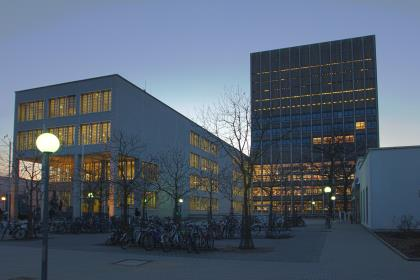
\includegraphics[width=\textwidth]{Abbildungen/bib.jpg}
	\caption{Außenansicht der KIT-Bibliothek. Bilder bitte immer manuell mit dem Parameter [h] setzen.	An dieser Stelle ist das Bild mit dem Figure-Parameter [h] platziert worden. Vor und nach der Figure-Umgebung steht eine Leerzeile.}
	\label{fig:bib}
\end{figure}

Lorem ipsum dolor sit amet, consetetur sadipscing elitr, sed diam nonumy eirmod tempor invidunt ut labore et dolore magna aliquyam erat, sed diam voluptua. At vero eos et accusam et justo duo dolores et ea rebum. Stet clita kasd gubergren, no sea takimata sanctus est Lorem ipsum dolor sit amet. Lorem ipsum dolor sit amet, consetetur sadipscing elitr, sed diam nonumy eirmod tempor invidunt ut labore et dolore magna aliquyam erat, sed diam voluptua. At vero eos et accusam et justo duo dolores et ea rebum. Stet clita kasd gubergren, no sea takimata sanctus est Lorem ipsum dolor sit amet.

Lorem ipsum dolor sit amet, consetetur sadipscing elitr, sed diam nonumy eirmod tempor invidunt ut labore et dolore magna aliquyam erat, sed diam voluptua. At vero eos et accusam et justo duo dolores et ea rebum. Stet clita kasd gubergren, no sea takimata sanctus est Lorem ipsum dolor sit amet. 	

%\newpage
\begin{figure}[h] % "\begin{figure}" ist eine Umgebung für Gleitobjekte, damit die Abbildung nummeriert und beschriftet ("\caption{}")und mit einem Label ("\label{fig:bib}") versehen und darauf verwiesen werden kann ("\ref{fig:bib}")
	\centering
%\hspace{-7pt} % Horizontale verschiebung der Bildreihe
	\subfloat[Subfloat. Bild Nr. 1. Zweizeilige Bildunterschriften stehen im Flattersatz.]{%
		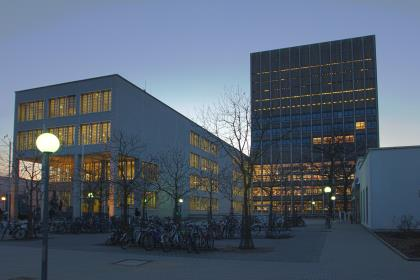
\includegraphics[width=0.49\linewidth]{Abbildungen/bib.jpg}%
	}
\hfill % Füllt den den vertikalen Abstand zwischen den Bildern auf, sofern die Bilder entsprechend klein sind
	\subfloat[Subfloat. Bild Nr. 2.]{%
		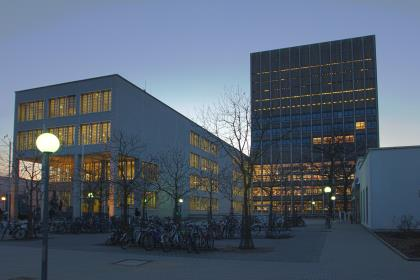
\includegraphics[width=0.49\linewidth]{Abbildungen/bib.jpg}%
	}
\\ \vspace{3mm} % Abstand zur zweiten Bildreihe % Plus Abstand aufgrund des Befehles "\captionsetup[subfloat]{belowskip=}" aus der Datei dokOptions.tex
%\hspace{-7pt} % Horizontale verschiebung der Bildreihe
	\subfloat[Subfloat. Bild Nr. 3. Mit linebreak \linebreak für einen manuellen Zeilenumbruch]{%
		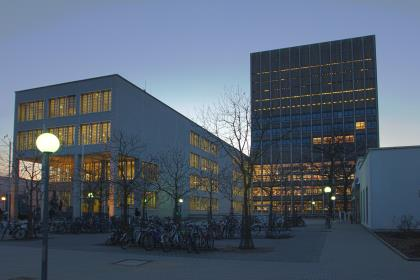
\includegraphics[width=0.49\linewidth]{Abbildungen/bib.jpg}%
	}
\hfill % Füllt den den vertikalen Abstand zwischen den Bildern auf, sofern die Bilder entsprechend klein sind
	\subfloat[Subfloat. Bild Nr. 4.]{%
		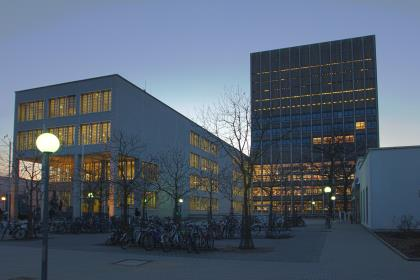
\includegraphics[width=0.49\linewidth]{Abbildungen/bib.jpg}%
	}
	\caption{Außenansicht der KIT-Bibliothek. Bilder bitte immer manuell mit dem Parameter [h] setzen.	An dieser Stelle ist das Bild mit dem Figure-Parameter [h] platziert worden. Vor und nach der Figure-Umgebung steht eine Leerzeile.}
	\label{fig:bib4}
\end{figure}

Lorem ipsum dolor sit amet, consetetur sadipscing elitr, sed diam nonumy eirmod tempor invidunt ut labore et dolore magna aliquyam erat, sed diam voluptua. At vero eos et accusam et justo duo dolores et ea rebum. Stet clita kasd gubergren, no sea takimata sanctus est Lorem ipsum dolor sit amet.

Curabitur a felis in nunc fringilla tristique. Morbi mattis ullamcorper velit. Phasellus gravida semper nisi. Nullam vel sem. Pellentesque libero tortor, tincidunt et, tincidunt eget, semper nec, quam. Sed hendrerit. Morbi ac felis. Nunc egestas, augue at pellentesque laoreet, felis eros vehicula leo, at malesuada velit leo quis pede. Donec interdum, metus et hendrerit aliquet, dolor diam sagittis ligula, eget egestas libero turpis vel mi. Nunc nulla. Fusce risus nisl, viverra et, tempor et.Pellentesque ut neque. Pellentesque habitant morbi tristique senectus et netus et malesuada fames ac turpis egestas. In dui magna, posuere eget, vestibulum et, tempor auctor, justo. In ac felis quis tortor malesuada pretium. Pellentesque auctor neque nec urna. Proin sapien ipsum, porta a, auctor quis, euismod ut, mi.

Aenean viverra rhoncus pede. Pellentesque habitant morbi tristique senectus et netus et malesuada fames ac turpis egestas. Ut non enim eleifend felis pretium feugiat vivamus quis mi. Phasellus a est. Phasellus magna. In hac habitasse platea dictumst. Curabitur at lacus ac velit ornare lobortis.\footnote{Cabo. Facerfe rferspient que nus molora doleserem. Ut a si autemo tectaquame enihil intota sam am ditati omnihil ma sequis re, aut fugiam earchil luptaque consequ.} Curabitur a felis in nunc fringilla tristique. Morbi mattis ullamcorper velit. Phasellus gravida semper nisi. Nullam vel sem. Pellentesque libero tortor, tincidunt et, tincidunt eget, semper nec, quam. Sed hendrerit.

%\newpage
Pellentesque habitant morbi tristique senectus et netus et malesuada fames ac turpis egestas. In dui magna, posuere eget, vestibulum et, tempor auctor, justo. In ac felis quis tortor malesuada pretium. Pellentesque auctor neque nec urna. Proin sapien ipsum, porta a, auctor quis, euismod ut, mi. Aenean viverra rhoncus pede. Pellentesque habitant morbi tristique senectus et netus et malesuada fames ac turpis egestas. Ut non enim eleifend felis pretium feugiat vivamus quis mi. Phasellus a est. Phasellus magna. In hac habitasse platea dictumst. Curabitur at lacus ac velit ornare lobortis. Aenean viverra rhoncus pede. Pellentesque habitant morbi tristique senectus et netus et malesuada fames ac turpis egestas. Ut non enim eleifend felis pretium feugiat vivamus quis mi. Phasellus a est. Phasellus magna. Phasellus a est. Phasellus magna. In hac habitasse platea dictumst. Curabitur at lacus ac velit ornare lobortis. Aenean viverra rhoncus pede. Pellentesque habitant morbi tristique senectus et netus et malesuada fames ac turpis egestas. Ut non enim eleifend felis pretium feugiat vivamus quis mi. Phasellus a est. Phasellus magna.

Phasellus magna. Phasellus a est. Phasellus magna. In hac habitasse platea dictumst. Curabitur at lacus ac velit ornare lobortis. Aenean viverra rhoncus pede. Pellentesque habitant morbi tristique senectus et netus et malesuada fames ac turpis egestas. Ut non enim eleifend felis pretium feugiat vivamus quis mi. Phasellus a est. Phasellus magna et netus et malesuada fames ac turpis egestas

%\newpage		 
\begin{figure}[h]
	\centering
	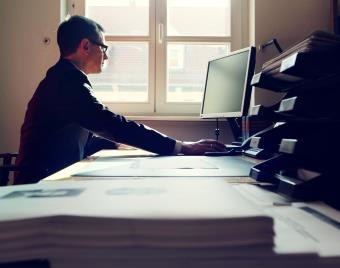
\includegraphics[width=6cm]{Abbildungen/wissen.jpg}
	\caption[Wissenschaftler an seinem Arbeitsplatz.]{Wissenschaftler an seinem Arbeitsplatz. Bilder bitte immer manuell mit dem Parameter [h] setzen. An dieser Stelle ist das Bild mit dem Figure-Parameter [h] platziert worden. Vor und nach der Figure-Umgebung steht eine Leerzeile.}
	\label{fig:wissen}
\end{figure}

Pellentesque habitant morbi tristique senectus et netus et malesuada fames ac turpis egestas. In dui magna, posuere eget, vestibulum et, tempor auctor, justo. In ac felis quis tortor malesuada pretium. Pellentesque auctor neque nec urna. Proin sapien ipsum, porta a, auctor quis, euismod ut, mi. Aenean viverra rhoncus pede. Pellentesque habitant morbi tristique senectus et netus et malesuada fames ac turpis egestas. Ut non enim eleifend felis pretium feugiat vivamus quis mi. Phasellus a est. Phasellus magna. In hac habitasse platea dictumst. Curabitur at lacus ac velit ornare lobortis.

Pellentesque habitant morbi tristique senectus et netus et malesuada fames ac turpis egestas. In dui magna, posuere eget, vestibulum et, tempor auctor, justo. In ac felis quis tortor malesuada pretium. Pellentesque auctor neque nec urna. Proin sapien ipsum, porta a, auctor quis, euismod ut, mi. Aenean viverra rhoncus pede. Pellentesque habitant morbi tristique senectus et netus et malesuada fames ac turpis egestas. Ut non enim eleifend felis pretium feugiat vivamus quis mi. Phasellus a est. Phasellus magna. In hac habitasse platea dictumst. Curabitur at lacus ac velit ornare lobortis. Pellentesque habitant morbi tristique senectus et netus et malesuada fames ac turpis egestas.

%Pellentesque habitant morbi tristique senectus et netus et malesuada fames ac turpis egestas. In dui magna, posuere eget, vestibulum et, tempor auctor. Pellentesque habitant morbi tristique senectus et netus et malesuada fames ac turpis egestas. In dui magna, posuere eget, vestibulum et, tempor auctor.

\begin{table}[h] % "\begin{table}" ist eine Umgebung für Gleitobjekte, damit die Tabelle "\begin{tabular}" nummeriert, übertitelt und mit einem Label versehen und darauf verwiesen werden kann
	\caption{Auch Tabellen ("table") werden immer mit dem Parameter [h] eingefügt. Vor und nach der Tabellen-Umgebung steht eine Leerzeile.}
	\begin{tabularx}{\textwidth}{XXXXXXXX} \toprule
		Spalte1 & Spalte2 & Spalte3 & Spalte4 & Spalte5
		& Spalte6 & Spalte7 & Spalte8 \\ \midrule
		AA      & BB      & CC      & DD      &
		EE      & FF      & GG      & HH       \\
		AA      & BB      & CC      & DD
		& EE      & FF      & GG      & HH    \\
		AA      & BB      & CC      & DD
		& EE      & FF      & GG      & HH    \\
		AA      & BB      & CC      & DD
		& EE      & FF      & GG      & HH    \\
		AA      & BB      & CC      & DD
		& EE      & FF      & GG      & HH    \\
		AA      & BB      & CC      & DD
		& EE      & FF      & GG      & HH     \\ \bottomrule
	\end{tabularx}
\end{table}

Pellentesque habitant morbi tristique senectus et netus et malesuada fames ac turpis egestas. In dui magna, posuere eget, vestibulum et, tempor auctor. Pellentesque habitant morbi tristique senectus et netus et malesuada fames ac turpis egestas. In dui magna, posuere eget, vestibulum et, tempor auctor.